% ------------------------------------------------------------------------------
% TYPO3 Version 10.4 - What's New (Italian Version)
%
% @license	Creative Commons BY-NC-SA 3.0
% @link		https://typo3.org/help/documentation/whats-new/
% @language	Italian
% ------------------------------------------------------------------------------

\section{Interfaccia utente di Backend}
\begin{frame}[fragile]
	\frametitle{Interfaccia utente di Backend}

	\begin{center}\huge{Capitolo 1:}\end{center}
	\begin{center}\huge{\color{typo3darkgrey}\textbf{Interfaccia utente di Backend}}\end{center}

\end{frame}

% ------------------------------------------------------------------------------
% ...

\begin{frame}[fragile]
	\frametitle{Interfaccia utente di Backend}
	\framesubtitle{Miglioramenti UI Backend}

	Interfaccia utente leggermente modificata nella colonna dei moduli di backend.

	\begin{figure}
		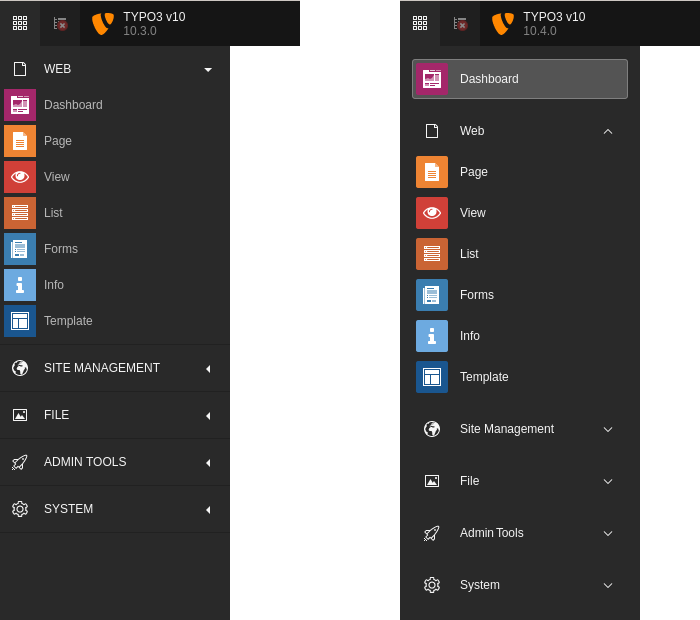
\includegraphics[width=0.5\linewidth]{BackendUserInterface/typo3-backend-ui.png}
	\end{figure}

\end{frame}

% ------------------------------------------------------------------------------
% Feature | 83128 | Content Element Filter

\begin{frame}[fragile]
	\frametitle{Interfaccia utente di Backend}
	\framesubtitle{Nuovo elemento di ricerca di contenuto}

	Gli utenti di backend possono ora cercare tipi di elementi di contenuto nella procedura guidata "Nuovo elemento di contenuto":

	\begin{figure}
		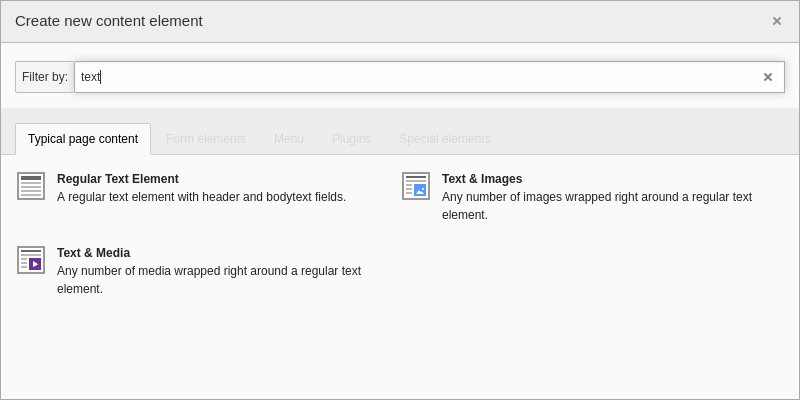
\includegraphics[width=0.6\linewidth]{BackendUserInterface/83128-ContentElementFilter.png}
	\end{figure}

\end{frame}

% ------------------------------------------------------------------------------
% Feature | 89513 | Provide password recovery for backend users

\begin{frame}[fragile]
	\frametitle{Interfaccia utente di Backend}
	\framesubtitle{Recupero Password}

	Gli utenti di backend possono ora richiedere un'e-mail per il recupero della password per ripristinare i dettagli di accesso.

	\begin{figure}
		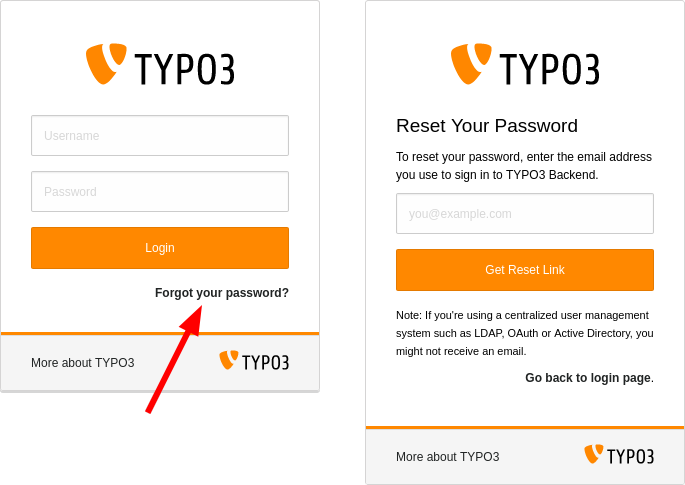
\includegraphics[width=0.6\linewidth]{BackendUserInterface/89513-ProvidePasswordRecoveryForBackendUsers.png}
	\end{figure}

\end{frame}

% ------------------------------------------------------------------------------
